% !TeX program = xelatex
% !BIB program = biber
\documentclass[light]{lutbeamer}

\usepackage{pgfpages}
\usepackage{ragged2e}
\usepackage{booktabs}
\usepackage{amssymb}
\usepackage{fontawesome5}
\usepackage{tikz}
\usepackage{pgfplots}
\pgfplotsset{compat=1.18}
\addbibresource{references.bib}

% ===================================================================
% METADATA (DERS KİMLİK BİLGİLERİ)
% ===================================================================
\setdepartment{OSTIM TECHNICAL UNIVERSITY}
\institute{}
\author[Faculty of Engineering]{\\
Prof.~Dr.~Yalçın ATA \\
Prof.~Dr.~Arif DEMİR \\
Dr.~Assist.~Prof.~Emel GÜVEN \\
Dr.~Assist.~Prof.~Ufuk ASIL \\
Lecturer Sema ÇİFTÇİ
}
\title{MATH 204 -- Probability and Statistics}
\subtitle{Week 3: Independence, Total Independence, Total Probability, Bayes' Theorem}
\date{2025--2026 Spring Semester}

% ===================================================================
% AUTOMATIC TABLE OF CONTENTS (PRESENTATION FLOW)
% ===================================================================
\setcounter{tocdepth}{2}

\AtBeginSection[]{
  \begin{frame}{Presentation Outline}
    \scriptsize
    \begin{columns}[T]
    \begin{column}{0.48\textwidth}
        \tableofcontents[sections={1-4}, currentsection]
      \end{column}
      \begin{column}{0.48\textwidth}
        \tableofcontents[sections={5-10}, currentsection]
      \end{column}
    \end{columns}
  \end{frame}
}

\begin{document}

\setbeamertemplate{navigation symbols}{}
\setbeamertemplate{footline}{
  \begin{beamercolorbox}[wd=\paperwidth, ht=10pt, dp=1pt]{footline}
    \usebeamerfont{footline}
    \begin{tikzpicture}[remember picture,overlay]
      \node[anchor=south west, xshift=10mm, yshift=.4mm]
      at (current page.south west)
      {\insertshortauthor,~\department};
    \end{tikzpicture}
    \begin{tikzpicture}[remember picture,overlay]
      \node[anchor=south east, xshift=-5mm, yshift=0.5mm]
      at (current page.south east)
      {\insertframenumber \,/\, \inserttotalframenumber};
    \end{tikzpicture}
  \end{beamercolorbox}
}

% ===================================================================
% KAPAK SLAYTLARI
% ===================================================================

% Görsel Tam Kapak (Logosuz)
\begin{frame}<article:0>[plain,noframenumbering]
    \begin{tikzpicture}[remember picture,overlay]
        \node[anchor=center, at=(current page.center), inner sep=0pt] {
            \includegraphics[width=\paperwidth, height=\paperheight]{logos/background_figure.jpg}
        };
    \end{tikzpicture}
\end{frame}

% Resmi Başlık Sayfası (kapak için özel alt bilgi)
{
  \setbeamertemplate{footline}{
    \begin{beamercolorbox}[wd=\paperwidth, ht=10pt, dp=1pt]{footline}
      \usebeamerfont{footline}
      \begin{tikzpicture}[remember picture,overlay]
        \node[anchor=south west, xshift=10mm, yshift=.4mm, align=left]
        at (current page.south west)
        {\tiny This template was prepared by OSTIM Technical University Software Engineering, and you can reach the current version \href{https://github.com/ufukasia/Ostim-Teknik--niversitesi-Yaz-l-m-M-hendisli-i---Lutbeamer-egitim-i-eri-i-haz-rlama-}{here}.};
      \end{tikzpicture}
      \begin{tikzpicture}[remember picture,overlay]
        \node[anchor=south east, xshift=-5mm, yshift=0.5mm]
        at (current page.south east)
        {\insertframenumber \,/\, \inserttotalframenumber};
      \end{tikzpicture}
    \end{beamercolorbox}
  }
  \maketitle{}
}

% GENEL İÇERİK HARİTASI
\begin{frame}{Contents}
  \scriptsize
  \begin{columns}[T]
    \begin{column}{0.48\textwidth}
      \tableofcontents[sections={1-4}]
    \end{column}
    \begin{column}{0.48\textwidth}
      \tableofcontents[sections={5-10}]
    \end{column}
  \end{columns}
\end{frame}

% ===================================================================
% ICERIK: HAFTA 3 - OLASILIK
% ===================================================================


\section{Bridge from Week 2}
\subsection{Recap and Learning Plan}

\begin{frame}{What Are We Bringing from Week 2?}
    \begin{block}{Basic Recap}
        The entirety of this week is built upon two ideas from last week:
        \[
        P(A|B)=\frac{P(A\cap B)}{P(B)}, \qquad
        P(A\cap B)=P(A)P(B|A).
        \]
    \end{block}

    \begin{itemize}
        \item Conditional probability: ``shrinking the universe'' to calculate.
        \item Multiplication rule: thinking sequentially about the probability of occurring together.
        \item This week: \textbf{Independence}, \textbf{Total Independence}, \textbf{Total Probability}, \textbf{Bayes}.
    \end{itemize}
\end{frame}

\subsection{Motivation: Updating Belief with a Single Evidence}

\begin{frame}{Motivation: ``Smiled'' \texorpdfstring{$\Rightarrow$}{->} ``Loves Me''?}
    \footnotesize
    \begin{columns}[T]
        \begin{column}{0.4\textwidth}
            \begin{block}{Hypothesis and evidence}
                \begin{itemize}
                    \item $A$: ``The person loves me''
                    \item $B$: ``Smiled at me''
                \end{itemize}
            \end{block}

            \begin{alertblock}{Warning: Most common fallacy}
                \[
                P(A\mid B)\ \text{(if smiled, does love?)}
                \]
                \[
                \neq\ P(B\mid A)\ \text{(if loves, will smile?)}
                \]
            \end{alertblock}

            \begin{block}{Bayes' rule}
                \[
                P(A\mid B)=\frac{P(B\mid A)\,P(A)}{P(B)}.
                \]
            \end{block}

        \end{column}

        \begin{column}{0.55\textwidth}
            \centering
            \includegraphics[width=1\textwidth,height=1\textheight,keepaspectratio]{figures/baes.png}
            \vspace{0.15cm}

            \tiny
            \vspace{-1cm}
            \textit{Iconic message: Update hypothesis (\(A\)) upon seeing evidence (\(B\)).}
        \end{column}
    \end{columns}
\end{frame}

\begin{frame}{Numerical Mini Example: Why is \texorpdfstring{$P(B)$}{P(B)} critical?}
    \small
    \begin{columns}[T]
        \begin{column}{0.58\textwidth}
            \begin{block}{Reasonable assumptions (for example)}
                \begin{itemize}
                    \item Prior: $P(A)=0.10$ \hfill (10\%: initial belief)
                    \item Evidence strength: $P(B\mid A)=0.70$ \hfill (smiling if loves)
                    \item Alternative: $P(B\mid A')=0.30$ \hfill (might smile even if doesn't love)
                \end{itemize}
            \end{block}

            \begin{block}{Denominator first: Total Probability}
                \[
                P(B)=P(B\mid A)P(A)+P(B\mid A')P(A').
                \]
            \end{block}

            \begin{itemize}
                \item In Bayes calculation, the denominator carries the ``general frequency'' of the evidence.
                \item If evidence is very common in the population, distinctiveness decreases.
            \end{itemize}
        \end{column}

        \begin{column}{0.38\textwidth}
            \begin{block}{Calculation}
                \footnotesize
                \[
                P(B)=0.70(0.10)+0.30(0.90)=0.34
                \]
                \[
                P(A\mid B)=\frac{0.70(0.10)}{0.34}=\frac{0.07}{0.34}\approx 0.206
                \]
            \end{block}

            \begin{alertblock}{Result}
                Probability rises from 10\% to \textbf{20.6\%} because of the smile;
                but it \textbf{does not become 70\%}.
            \end{alertblock}

            \tiny
            \textit{A single piece of evidence updates belief; it does not produce immediate ``certainty''.}
        \end{column}
    \end{columns}
\end{frame}

\begin{frame}{From this iconic example to the Theorem: The Chain of the Week}
    \footnotesize
    \begin{columns}[T]
        \begin{column}{0.58\textwidth}
            \begin{block}{Reading Bayes without memorization}
                \[
                P(A\mid B)=\frac{P(A\cap B)}{P(B)}
                \]
                \begin{itemize}
                    \item Numerator: ``Both $A$ and $B$'' (relevant path)
                    \item Denominator: ``All paths producing $B$'' (total)
                \end{itemize}
            \end{block}

            \begin{block}{Why together this week?}
                \[
                \begin{aligned}
                    \text{Multiplication:}\quad & P(A\cap B)=P(A)P(B\mid A) \\
                    \text{Total:}\quad & P(B)=P(B\mid A)P(A)+P(B\mid A')P(A') \\
                    \text{Bayes:}\quad & P(A\mid B)=\frac{P(A\cap B)}{P(B)}
                \end{aligned}
                \]
            \end{block}
        \end{column}

        \begin{column}{0.38\textwidth}
            \begin{alertblock}{Lecture message (one sentence)}
                When you see evidence, first choose the correct direction: \\
                \(P(A\mid B)\) or \(P(B\mid A)\)?
                Then count \textbf{all paths} in the denominator.
            \end{alertblock}

        \end{column}
    \end{columns}
\end{frame}

\begin{frame}{Learning Objectives of This Week}
    \begin{enumerate}
        \item Correctly distinguishing between independence and disjointness.
        \item Demonstrating the difference between pairwise independence and total independence with an example.
        \item Calculating the general probability of an event using Total Probability.
        \item Making inference ``from effect to cause'' using Bayes' Theorem.
        \item Selecting the correct method in a question and producing a systematic solution.
    \end{enumerate}
\end{frame}

\begin{frame}{4-Step Routine for Home Study}
    \begin{block}{Same order in every question}
        \begin{enumerate}
            \item Symbolize the events.
            \item Diagnose the question type (Intersection/Total/Bayes).
            \item Check the precondition of the formula (partition, independence, positivity).
            \item Interpret the numerical result in context.
        \end{enumerate}
    \end{block}
\end{frame}

\begin{frame}{Flow Logic: Why This Order?}
    \begin{enumerate}
        \item Base: \(P(A\cap B)=P(A)P(B|A)\) (multiplication rule).
        \item Shortcut in independence: \(P(B|A)=P(B)\Rightarrow P(A\cap B)=P(A)P(B)\).
        \item General probability in multiple scenarios: \(P(A)=\sum_i P(B_i)P(A|B_i)\) (Total Probability).
        \item Returning from observation to source: Bayes and \(P(B_r|A)\).
    \end{enumerate}
\end{frame}

\section{Independent Events}
\subsection{Definition, Intuition, and Application}

\begin{frame}{Definition of Independence (Definition 2.11)}
    \begin{block}{Definition}
        Two events \(A\) and \(B\) are independent if
        \[
        P(A\cap B)=P(A)P(B).
        \]
    \end{block}

    \begin{itemize}
        \item Equivalent expression (when denominators are positive): \(P(A|B)=P(A)\), \(P(B|A)=P(B)\)
        \item Intuition: Knowledge of one event does not change the probability of the other.
        \item \textbf{Important result:} If $A$ and $B$ are independent, then $A'$ and $B$,\; $A$ and $B'$,\; $A'$ and $B'$ are also independent.
    \end{itemize}

    \begin{block}{One-line proof (for $A'$ and $B$)}
        \[
        P(A'\cap B)=P(B)-P(A\cap B)=P(B)-P(A)P(B)=P(B)(1-P(A))=P(A')P(B) \;\checkmark
        \]
    \end{block}
\end{frame}

\begin{frame}{Disjoint or Independent?}
    \begin{columns}[T]
        \begin{column}{0.48\textwidth}
            \textbf{Disjoint (Mutually Exclusive)}
            \begin{itemize}
                \item \(A\cap B=\emptyset\)
                \item \(P(A\cap B)=0\)
                \item Contradicts independence for two events with positive probability
            \end{itemize}
            \centering
            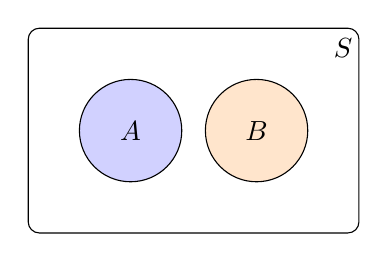
\begin{tikzpicture}[x=1cm,y=1cm]
                \draw[rounded corners] (0,0) rectangle (4.2,2.6);
                \node at (4.0,2.35) {$S$};
                \draw[fill=blue!18] (1.3,1.3) circle (0.65);
                \draw[fill=orange!20] (2.9,1.3) circle (0.65);
                \node at (1.3,1.3) {$A$};
                \node at (2.9,1.3) {$B$};
            \end{tikzpicture}
        \end{column}
        \begin{column}{0.48\textwidth}
            \textbf{Independent}
            \begin{itemize}
                \item \(P(A\cap B)=P(A)P(B)\)
                \item Intersection does not have to be empty
                \item No information effect
            \end{itemize}
            \centering
            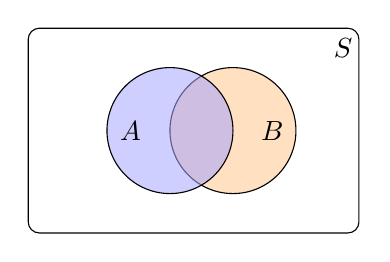
\begin{tikzpicture}[x=1cm,y=1cm]
                \draw[rounded corners] (0,0) rectangle (4.2,2.6);
                \node at (4.0,2.35) {$S$};
                \draw[fill=orange!45, fill opacity=0.55] (2.6,1.3) circle (0.8);
                \draw[fill=blue!35, fill opacity=0.55] (1.8,1.3) circle (0.8);
                \node at (1.3,1.3) {$A$};
                \node at (3.1,1.3) {$B$};
            \end{tikzpicture}
        \end{column}
    \end{columns}

    \vspace{0.15cm}
    \begin{block}{Why the contradiction?}
        If disjoint, $P(A\cap B)=0$, but independence requires $P(A)P(B)>0$. $0 \neq P(A)P(B)$ $\Rightarrow$ contradiction.
    \end{block}
\end{frame}

\begin{frame}{Concrete Example: Disjointness vs Independence}
    \begin{columns}[T]
        \begin{column}{0.48\textwidth}
            \begin{block}{\faLink\ Disjoint Events}
                \textbf{\textit{``If this happened, the other CANNOT happen''}}
                \vspace{0.2cm}
                
                \textbf{Scenario:} Status of a car.
                \begin{itemize}
                    \item \(A\): Car is working.
                    \item \(B\): Car is completely broken.
                \end{itemize}
                
                \textbf{Analysis:}
                \begin{itemize}
                    \item A car cannot be working and broken at the same time.
                    \item Intersection is IMPOSSIBLE ($P(A\cap B)=0$).
                    \item Knowing one affects the other 100\% (If broken, it is not working).
                \end{itemize}
            \end{block}
        \end{column}
        \begin{column}{0.48\textwidth}
            \begin{block}{\faUnlink\ Independent Events}
                \textbf{\textit{``If this happened, it DOES NOT MATTER for the other''}}
                \vspace{0.2cm}
                
                \textbf{Scenario:} Status of two different cars.
                \begin{itemize}
                    \item \(A\): Car in Istanbul is working.
                    \item \(B\): Car in Ankara is broken.
                \end{itemize}
                
                \textbf{Analysis:}
                \begin{itemize}
                    \item Status in Istanbul does not affect Ankara.
                    \item Both can happen at the same time ($P(A\cap B) \neq 0$).
                    \item Knowing one provides no information about the other.
                \end{itemize}
            \end{block}       
        \end{column}
    \end{columns}
\end{frame}

\begin{frame}[fragile]{Multiplication Rule in Independence}
    General multiplication:
    \[
    P(A\cap B)=P(A)P(B|A)
    \]
    In independence:
    \[
    P(B|A)=P(B)\quad \Rightarrow\quad P(A\cap B)=P(A)P(B).
    \]

    \begin{block}{Quick Test}
        If \(P(A\cap B)\) equals \(P(A)P(B)\) from the data, there is independence.
    \end{block}
\end{frame}

\begin{frame}{Example 2.38: Firefighter and Ambulance}
    \small
    In a small town, there is one fire truck and one ambulance. The probabilities of the vehicles being available in case of an emergency are independent:
    \begin{itemize}
        \item Probability of fire truck being available: $P(I) = 0.98$
        \item Probability of ambulance being available: $P(A) = 0.92$
    \end{itemize}

    \only<1>{
        \footnotesize
        \begin{block}{Solution Skeleton}
            The target event is \(I \cap A\). Since independence is given, we directly use
            \(P(I \cap A)=P(I)P(A)\).
        \end{block}
    }

    \vspace{0.2cm}
    \textbf{Question:} What is the probability that \textbf{both} vehicles are available at the time of an accident?

    \onslide<2->{
        \textbf{Solution:} Since the events are independent, intersection equals multiplication:
        \[ P(I \cap A) = P(I) \cdot P(A) \]
        \[ P(I \cap A) = (0.98)(0.92) = 0.9016 \]
    }
\end{frame}

\subsection{Reinforcement Questions (Your Turn)}

\begin{frame}{Question 2: Backup Power Unit (Independence)}
    A data center has two independent backup power units (Generator A and Generator B).
    \begin{itemize}
        \item Probability of Generator A working successfully: $P(A) = 0.90$
        \item Probability of Generator B working successfully: $P(B) = 0.80$
    \end{itemize}

    \textbf{Question:} In case of a power outage;
    \begin{enumerate}
        \item[(a)] What is the probability that both generators work at the same time ($A \cap B$)?
        \item[(b)] What is the probability that the system is completely out of power (both fail)?
        \item[(c)] What is the probability that at least one generator works ($A \cup B$)?
    \end{enumerate}
\end{frame}

\begin{frame}{Question 2: Solution}
    \vspace{5cm}
\end{frame}

\begin{frame}[allowframebreaks]{Question 2: Detailed Solution}
    \small
    {\color{red}
    \textbf{Given:} \(P(A)=0.90\), \(P(B)=0.80\), events are independent.

    \textbf{(a) Both generators working}
    \[
    P(A\cap B)=P(A)P(B)=(0.90)(0.80)=\mathbf{0.72}
    \]

    \textbf{(b) System completely out of power}
    \[
    P(A')=0.10,\qquad P(B')=0.20
    \]
    Independence carries over to complements:
    \[
    P(A'\cap B')=P(A')P(B')=(0.10)(0.20)=\mathbf{0.02}
    \]

    \textbf{(c) At least one generator working}
    \[
    P(A\cup B)=1-P(A'\cap B')=1-0.02=\mathbf{0.98}
    \]

    \textbf{Result:} In case of an outage, the system provides power with at least one source with \(\%98\) probability.
    }
\end{frame}



\begin{frame}{Independence Checklist}
    \begin{enumerate}
        \item \textbf{Do not assume automatically:} Do not assume independence unless explicitly stated ``independent'' in the question.
        \item \textbf{Disjointness $\neq$ Independence:} Disjoint events ($A\cap B=\emptyset$) cannot be independent if they have positive probability.
        \item \textbf{Perform numerical test:} If you have enough data, directly check the equality \(P(A\cap B)\stackrel{?}{=}P(A)P(B)\).
    \end{enumerate}
\end{frame}

\begin{frame}{How to Test Numerically? (Examples)}
    \begin{columns}[T]
        \begin{column}{0.48\textwidth}
            \begin{exampleblock}{Example 1: Independence Exists}
                \small
                \textbf{Data:} $P(A)=0.4$, $P(B)=0.5$, $P(A \cap B)=0.2$.
                
                \textbf{Test:}
                \[ P(A) \cdot P(B) \stackrel{?}{=} P(A \cap B) \]
                \[ 0.4 \cdot 0.5 = 0.2 \]
                \[ 0.2 = 0.2 \quad \text{\faCheck} \]
                
                \textbf{Result:} Since equality holds, events are \textbf{independent}.
            \end{exampleblock}
        \end{column}
        \begin{column}{0.48\textwidth}
            \begin{alertblock}{Example 2: Dependence Exists}
                \small
                \textbf{Data:} $P(A)=0.4$, $P(B)=0.5$, $P(A \cap B)=0.1$.
                
                \textbf{Test:}
                \[ P(A) \cdot P(B) \stackrel{?}{=} P(A \cap B) \]
                \[ 0.4 \cdot 0.5 = 0.2 \]
                \[ 0.2 \neq 0.1 \quad \text{\faTimes} \]
                
                \textbf{Result:} Since equality is broken, events are \textbf{dependent}.
            \end{alertblock}
        \end{column}
    \end{columns}
\end{frame}

\section{Total Independence}
\subsection{Pairwise Independence and Total Independence}

\begin{frame}{Why is Pairwise Independence Not Enough?}
    For three events \(A,B,C\), having only
    \[
    P(A\cap B)=P(A)P(B),\;
    P(A\cap C)=P(A)P(C),\;
    P(B\cap C)=P(B)P(C)
    \]
    is not sufficient.

    \begin{block}{Total Independence}
        Multiplication rule must hold for every subset.
    \end{block}
\end{frame}

\begin{frame}{Definition: Mutual Independence (Definition 2.12)}
    All conditions required for three events:
    \begin{enumerate}
        \item \(P(A\cap B)=P(A)P(B)\)
        \item \(P(A\cap C)=P(A)P(C)\)
        \item \(P(B\cap C)=P(B)P(C)\)
        \item \(P(A\cap B\cap C)=P(A)P(B)P(C)\)
    \end{enumerate}

    \begin{block}{Generalization}
        Total independence for $n$ events requires a total of $2^n - n - 1$ conditions.\\
        \textbf{Examples:} 3~events $\rightarrow$ 4~conditions,\quad 4~events $\rightarrow$ 11~conditions,\quad 5~events $\rightarrow$ 26~conditions.\\
        Just pairwise equalities (1--3) are not enough; triple (4) must also be satisfied.
    \end{block}
\end{frame}

\begin{frame}[fragile]{Counter-Example: Pairwise Independence Exists, Total Does Not}
    \footnotesize
    \begin{columns}[T,onlytextwidth]
        \begin{column}{0.49\textwidth}
            \textbf{Experiment Definition:} Two fair coin tosses, \(S=\{HH,HT,TH,TT\}\).\\
            \textit{Note:} \(H\)=Heads, \(T\)=Tails.
            \[
            A=\{\text{first toss }H\},\quad
            B=\{\text{second toss }H\},\quad
            C=\{\text{two tosses same}\}
            \]

            \textbf{Probabilities:}
            \begin{itemize}\itemsep2pt
                \item \(P(A)=P(B)=P(C)=\tfrac{1}{2}\)
                \item \(P(A\cap B)=P(A\cap C)=P(B\cap C)=\tfrac{1}{4}\)
            \end{itemize}
            All pairwise combinations are independent.
        \end{column}
        \begin{column}{0.49\textwidth}
            \begin{alertblock}{Triple Intersection Analysis}
                \textbf{Why \(P(A \cap B \cap C)=\tfrac{1}{4}\)?}
                \begin{itemize}\itemsep2pt
                    \item \(A \cap B = \{HH\}\)
                    \item When \(HH\) occurs, \(C\) is automatically satisfied.
                    \item \((A \cap B) \cap C = \{HH\}\)
                \end{itemize}
                \[
                P(A \cap B \cap C)=\tfrac{1}{4},\qquad
                P(A)P(B)P(C)=\tfrac{1}{8}
                \]
                \[
                \tfrac{1}{4} \neq \tfrac{1}{8}\Rightarrow \text{not totally independent.}
                \]
            \end{alertblock}
        \end{column}
    \end{columns}

    \[
    \boxed{\text{Pairwise independence exists, total independence does not.}}
    \]
\end{frame}

\begin{frame}{Example 2.39: Series and Parallel Circuits}
    \begin{columns}[T]
        \begin{column}{0.55\textwidth}
            \textbf{Question:}
            In a circuit as shown in the figure, probabilities of components working are $P(C_1)=0.9$, $P(C_2)=0.9$, $P(C_3)=0.8$ and are independent of each other. What is the probability of the circuit (system) working?

            \vspace{0.2cm}
            \centering
            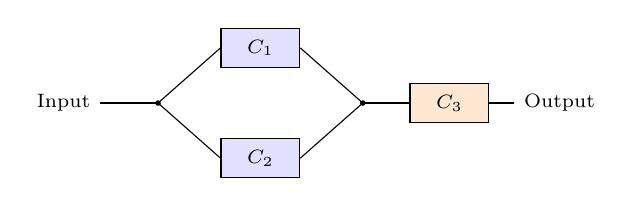
\begin{tikzpicture}[x=1cm,y=1cm,>=stealth,every node/.style={font=\scriptsize}]
                % Nodes where branches split and merge
                \coordinate (split) at (1.2,0.5);
                \coordinate (merge) at (3.8,0.5);

                % Components (C1 and C2 symmetric around center)
                \node[draw, fill=blue!12, minimum width=1cm, minimum height=0.5cm] (c1) at (2.5,1.2) {$C_1$};
                \node[draw, fill=blue!12, minimum width=1cm, minimum height=0.5cm] (c2) at (2.5,-0.2) {$C_2$};
                \node[draw, fill=orange!18, minimum width=1cm, minimum height=0.5cm] (c3) at (4.9,0.5) {$C_3$};

                % Input/Output labels
                \node (in) at (0,0.5) {Input};
                \node (out) at (6.3,0.5) {Output};

                % Connections (using anchor to touch boxes perfectly)
                \draw (in.east) -- (split);
                \draw (split) -- (c1.west);
                \draw (split) -- (c2.west);
                \draw (c1.east) -- (merge);
                \draw (c2.east) -- (merge);
                \draw (merge) -- (c3.west);
                \draw (c3.east) -- (out.west);

                % Make nodes visible
                \fill (split) circle (1pt);
                \fill (merge) circle (1pt);
            \end{tikzpicture}
        \end{column}
        \begin{column}{0.44\textwidth}
            \onslide<2->{
                \textbf{Solution:}
                \small
                \begin{itemize}
                    \item \textbf{Parallel Part ($A$):} $C_1 \cup C_2$.
                    $P(A) = 1 - P(C_1' \cap C_2')$
                    $P(A) = 1 - (0.1)(0.1) = 0.99$.

                    \item \textbf{Entire System:} $A \cap C_3$ (Series).
                    $A$ is a function of events $(C_1,C_2)$ only; since $C_3$ is given as independent of these two, $A$ and $C_3$ are independent.
                    $P(\text{System}) = P(A) \cdot P(C_3)$
                    $P(\text{System}) = 0.99 \cdot 0.8 = 0.792$.
                \end{itemize}
            }
        \end{column}
    \end{columns}
\end{frame}

\subsection{Practice Questions (Your Turn)}

\begin{frame}{Question 3: Advanced System Reliability}
    \small
    A system with five components ($K_1 - K_5$) has the following structure:
    \begin{itemize}
        \item \textbf{Main Structure:} Three main branches ($Branch_1, Branch_2, Branch_3$) are \textbf{parallel} to each other.
        \item \textbf{Branch 1:} Component $K_1$ is connected in \textbf{series} to a block (where $K_2$ and $K_3$ are parallel).
        \item \textbf{Branch 2:} Contains only component $K_4$.
        \item \textbf{Branch 3:} Contains only component $K_5$.
    \end{itemize}

    \textbf{Failure Probabilities (Independent):}
    $P(K_1')=0.05, P(K_2')=0.10, P(K_3')=0.10, P(K_4')=0.20, P(K_5')=0.20$.

    \vspace{0.2cm}
    \begin{columns}[T]
        \begin{column}{0.45\textwidth}
            \textbf{Questions:}
            \begin{enumerate}
                \item[(a)] What is the probability of the system \textbf{COMPLETELY failing}?
                \item[(b)] What is the probability of the system \textbf{working}?
            \end{enumerate}
        \end{column}
        \begin{column}{0.50\textwidth}
            \centering
            % TikZ Circuit Diagram
            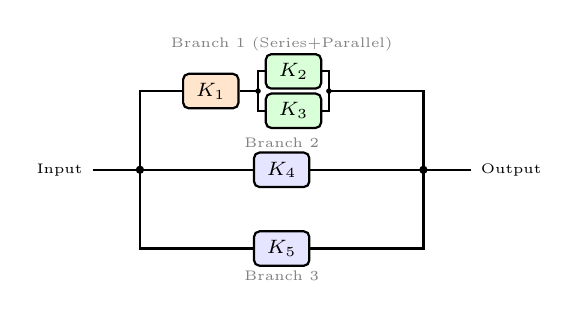
\begin{tikzpicture}[x=0.6cm,y=0.5cm,>=stealth, line width=0.8pt]
                \tikzstyle{block} = [draw, fill=blue!10, rectangle, minimum height=1.2em, minimum width=2em, rounded corners=2pt, font=\scriptsize]
                
                % Input Node
                \coordinate (input) at (0,0);
                \coordinate (split) at (1,0);
                \coordinate (merge) at (7,0);
                \coordinate (output) at (8,0);

                % Main Lines
                \draw (input) -- (split);
                \draw (merge) -- (output) node[right] {\tiny Output};
                \draw (input) node[left] {\tiny Input};

                % Branch 1 (Top - Complex)
                \draw (split) -- (1, 2) -- (2, 2);
                \node[block, fill=orange!20] (k1) at (2.5, 2) {$K_1$};
                \draw (k1.east) -- (3.5, 2);
                
                % Branch 1 - Parallel Subpart
                % Create nodes first
                \node[block, fill=green!15] (k2) at (4.25, 2.5) {$K_2$};
                \node[block, fill=green!15] (k3) at (4.25, 1.5) {$K_3$};
                
                % Then draw lines (so lines appear above nodes)
                \draw (3.5, 2) -- (3.5, 2.5) -- (k2.west);
                \draw (k2.east) -- (5, 2.5) -- (5, 2);

                \draw (3.5, 2) -- (3.5, 1.5) -- (k3.west);
                \draw (k3.east) -- (5, 1.5) -- (5, 2);
                
                \draw (5, 2) -- (7, 2) -- (merge);

                % Branch 2 (Middle - Simple)
                \node[block] (k4) at (4, 0) {$K_4$};
                \draw (split) -- (k4.west);
                \draw (k4.east) -- (merge);

                % Branch 3 (Bottom - Simple)
                \draw (split) -- (1, -2) -- (3.5, -2);
                \node[block] (k5) at (4, -2) {$K_5$};
                \draw (k5.east) -- (7, -2) -- (merge);

                % Labels
                \node[font=\tiny, gray] at (4, 3.2) {Branch 1 (Series+Parallel)};
                \node[font=\tiny, gray] at (4, 0.7) {Branch 2};
                \node[font=\tiny, gray] at (4, -2.7) {Branch 3};

                % Node points
                \fill[black] (split) circle (1.5pt);
                \fill[black] (merge) circle (1.5pt);
                \fill[black] (3.5, 2) circle (1pt);
                \fill[black] (5, 2) circle (1pt);
            \end{tikzpicture}
        \end{column}
    \end{columns}
\end{frame}

\begin{frame}[allowframebreaks]{Question 3: Detailed Solution}
    \small
    {\color{red}
    \textbf{Strategy:} Since the system consists of parallel main branches, the system \textbf{failing} means \textbf{ALL branches} failing simultaneously.
    \[ P(S') = P(Branch_1') \times P(Branch_2') \times P(Branch_3') \]

    \textbf{Step 1: Analysis of Branch 1}
    \begin{itemize}
        \item $K_2$ and $K_3$ parallel: $P(\text{subpart failed}) = P(K_2')P(K_3') = (0.10)(0.10) = 0.01$.
        \item This subgroup ($0.01$) is connected in \textbf{series} with $K_1$ ($0.05$).
        \item In series structure, we multiply probabilities of \textbf{working}:
        \[ R_{sub} = 1 - 0.01 = 0.99, \quad R_{K1} = 1 - 0.05 = 0.95 \]
        \[ R_{Branch1} = 0.95 \times 0.99 = 0.9405 \]
        \item Branch 1 Failure: $P(Branch_1') = 1 - 0.9405 = \mathbf{0.0595}$.
    \end{itemize}

    \textbf{Step 2: Other Branches}
    \begin{itemize}
        \item $P(Branch_2') = P(K_4') = \mathbf{0.20}$
        \item $P(Branch_3') = P(K_5') = \mathbf{0.20}$
    \end{itemize}

    \textbf{Step 3: System Result}
    \[
    \textbf{(a) } P(S') = (0.0595) \times (0.20) \times (0.20) = 0.0595 \times 0.04 = \mathbf{0.00238}
    \]
    \[
    \textbf{(b) } P(S) = 1 - P(S') = 1 - 0.00238 = \mathbf{0.99762}
    \]
    
    So the system is approximately \textbf{99.76\%} reliable.
    }
\end{frame}

\section{Total Probability Theorem}
\subsection{Partition and Theorem}

\begin{frame}{What is a Partition?}
    \begin{columns}[T]
        \begin{column}{0.58\textwidth}
            \begin{block}{Definition}
                If sample space \(S\) is partitioned by events \(B_1,\dots,B_k\):
                \begin{enumerate}
                    \item \(B_i\cap B_j=\emptyset\) for \(i\neq j\),
                    \item \(\bigcup_{i=1}^{k} B_i=S\),
                    \item \(P(B_i)>0\) for every \(i\).
                \end{enumerate}
            \end{block}
            \textbf{Goal:} To split a complex event into non-overlapping sub-scenarios.
        \end{column}
        \begin{column}{0.40\textwidth}
            \centering
            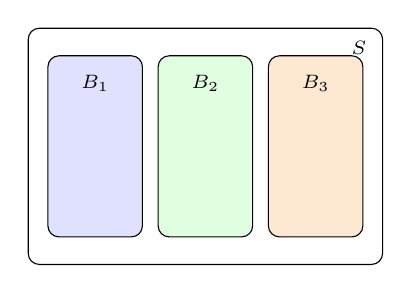
\begin{tikzpicture}[x=1cm,y=1cm,every node/.style={font=\scriptsize}]
                \draw[rounded corners] (0,0) rectangle (4.5,3.0);
                \node at (4.2,2.75) {$S$};
                \draw[fill=blue!12,rounded corners] (0.25,0.35) rectangle (1.45,2.65);
                \draw[fill=green!12,rounded corners] (1.65,0.35) rectangle (2.85,2.65);
                \draw[fill=orange!18,rounded corners] (3.05,0.35) rectangle (4.25,2.65);
                \node at (0.85,2.3) {$B_1$};
                \node at (2.25,2.3) {$B_2$};
                \node at (3.65,2.3) {$B_3$};
            \end{tikzpicture}
        \end{column}
    \end{columns}
\end{frame}

\begin{frame}{Partitioning of Events}
    Any event $A$ can be written as a union of intersections with partition elements:
    \[
    A = (B_1 \cap A) \cup (B_2 \cap A) \cup \cdots \cup (B_k \cap A)
    \]

    Since these intersections ($B_i \cap A$) are \textbf{disjoint} from each other, the total probability of $A$ is the sum of the probabilities of these parts:
    \[
    P(A) = P(B_1 \cap A) + P(B_2 \cap A) + \cdots + P(B_k \cap A)
    \]

    \begin{block}{Next step}
        If we expand each $P(B_i \cap A)$ term using the multiplication rule, we reach the Total Probability Theorem.
    \end{block}
\end{frame}

\begin{frame}[fragile]{Total Probability Theorem (Theorem 2.13)}
    \begin{block}{Theorem}
        If \(B_1,\dots,B_k\) is a partition:
        \[
        P(A)=\sum_{i=1}^{k}P(B_i\cap A)=\sum_{i=1}^{k}P(B_i)P(A|B_i).
        \]
    \end{block}

    \begin{itemize}
        \item Each term: ``branch probability'' (\(P(B_i)\times P(A|B_i)\)).
        \item Sum: Total of all paths leading to \(A\).
    \end{itemize}
\end{frame}


\begin{frame}{Example 2.41: Assembly Factory}
    \small
    \begin{columns}[T]
        \begin{column}{0.55\textwidth}
            \textbf{Question:}
            Three machines ($B_1, B_2, B_3$) are producing in a factory.
            \begin{itemize}
                \item Production shares: $B_1: \%30, \, B_2: \%45, \, B_3: \%25$.
                \item Defective product ($A$) rates: $P(A|B_1)=0.02,\; P(A|B_2)=0.03,\; P(A|B_3)=0.02$.
            \end{itemize}
            What is the probability that a randomly selected product is \textbf{defective}?
            
            \onslide<2->{
                \vspace{0.3cm}
                \footnotesize
                \textbf{Notation Analysis:}
                \begin{itemize}
                    \item $B_1, B_2, B_3$: Events of product coming from machines.
                    \item $A$: Event of selected product being \textbf{defective}.
                    \item $P(B_1)=0.30$: Production share of Machine 1.
                    \item $P(A|B_1)=0.02$: Defect rate under the condition that only Machine 1 produced it.
                \end{itemize}
            }
        \end{column}
        \begin{column}{0.44\textwidth}
            \only<1-2>{
                \footnotesize
                \begin{block}{Solution Skeleton}
                    Partition check $\rightarrow$
                    apply $P(A)=\sum_i P(B_i)P(A|B_i)$ $\rightarrow$
                    compare term contributions.
                \end{block}
            }

            \onslide<3->{
                \textbf{Solution:}
                Let's apply the Total Probability Theorem:
                \[ P(A) = \sum P(B_i)P(A|B_i) \]

                \footnotesize
                \begin{align*}
                P(A)&=0.30(0.02)+0.45(0.03)+0.25(0.02)\\
                    &=0.0245
                \end{align*}
                \[
                \mathbf{P(A)=0.0245=\%2.45}
                \]
            }
        \end{column}
    \end{columns}
\end{frame}




\begin{frame}{Total Probability: Reading Tree Diagram}
    \begin{columns}[T]
        \begin{column}{0.48\textwidth}
            \begin{block}{Path logic}
                Event $A$ can come from different sources ($B_1,B_2,B_3$):
                \[
                P(A)=\sum_i P(B_i)P(A|B_i).
                \]
                Each term is the \textbf{product} probability of a branch in the tree.
            \end{block}
            \begin{itemize}
                \item First, ``which source?'' branch is selected.
                \item Then, ``did $A$ happen in that source?'' branch is selected.
                \item All paths leading to $A$ are summed.
            \end{itemize}
        \end{column}
        \begin{column}{0.48\textwidth}
            \centering
            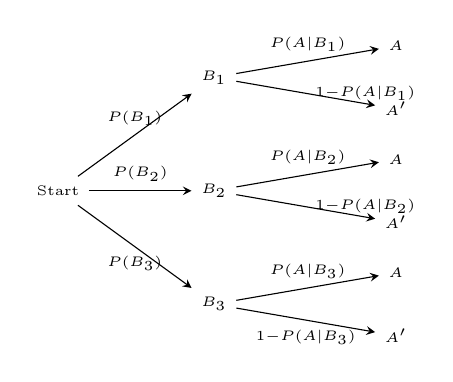
\begin{tikzpicture}[x=1.1cm,y=0.8cm,>=stealth, every node/.style={font=\tiny}]
                \node (r) at (0,0) {Start};
                \node (b1) at (1.8,1.8) {$B_1$};
                \node (b2) at (1.8,0.0) {$B_2$};
                \node (b3) at (1.8,-1.8) {$B_3$};

                \draw[->] (r)--(b1) node[midway,above] {$P(B_1)$};
                \draw[->] (r)--(b2) node[midway,above] {$P(B_2)$};
                \draw[->] (r)--(b3) node[midway,below] {$P(B_3)$};

                \node (a1) at (3.9,2.3) {$A$};
                \node (c1) at (3.9,1.3) {$A'$};
                \node (a2) at (3.9,0.5) {$A$};
                \node (c2) at (3.9,-0.5) {$A'$};
                \node (a3) at (3.9,-1.3) {$A$};
                \node (c3) at (3.9,-2.3) {$A'$};

                \draw[->] (b1)--(a1) node[midway,above] {$P(A|B_1)$};
                \draw[->] (b1)--(c1) node[midway,right] {$1{-}P(A|B_1)$};
                \draw[->] (b2)--(a2) node[midway,above] {$P(A|B_2)$};
                \draw[->] (b2)--(c2) node[midway,right] {$1{-}P(A|B_2)$};
                \draw[->] (b3)--(a3) node[midway,above] {$P(A|B_3)$};
                \draw[->] (b3)--(c3) node[midway,below] {$1{-}P(A|B_3)$};
            \end{tikzpicture}
        \end{column}
    \end{columns}
\end{frame}

% ------------------------------------------------------------
% QUESTION: Tree diagram (removal event A)
% ------------------------------------------------------------
\begin{frame}{Example: Tree Diagram (Quality Control)}
\small
\begin{columns}[T]
\begin{column}{0.48\textwidth}
Items coming off a production line:
\[
B_1:\ \text{highly defective},\quad
B_2:\ \text{slightly defective},\quad
B_3:\ \text{flawless}.
\]

Prior probabilities:
\[
P(B_1)=0.05,\quad P(B_2)=0.10,\quad P(B_3)=0.85.
\]

Workers remove the items they view as defective from the line:
\[
A:\ \text{``taken off the line''}.
\]

Conditional probabilities (from the diagram):
\[
P(A\mid B_1)=0.98,\quad P(A\mid B_2)=0.40,\quad P(A\mid B_3)=0.01.
\]
\end{column}

\begin{column}{0.48\textwidth}
\textbf{Question:} For an item removed from the line, find
\(\,P(B_1\mid A),\,P(B_2\mid A),\,P(B_3\mid A)\,\).

\centering
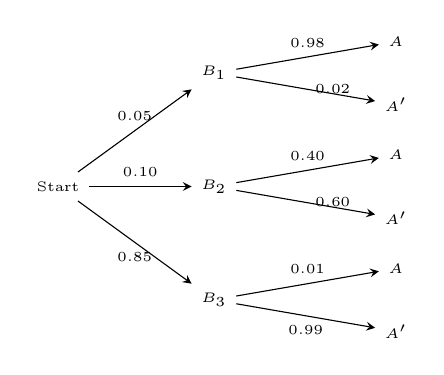
\begin{tikzpicture}[x=1.1cm,y=0.8cm,>=stealth, every node/.style={font=\tiny}]
    \node (r) at (0,0) {Start};
    \node (b1) at (1.8,1.8) {$B_1$};
    \node (b2) at (1.8,0.0) {$B_2$};
    \node (b3) at (1.8,-1.8) {$B_3$};

    \draw[->] (r)--(b1) node[midway,above] {$0.05$};
    \draw[->] (r)--(b2) node[midway,above] {$0.10$};
    \draw[->] (r)--(b3) node[midway,below] {$0.85$};

    \node (a1) at (3.9,2.3) {$A$};
    \node (c1) at (3.9,1.3) {$A'$};
    \node (a2) at (3.9,0.5) {$A$};
    \node (c2) at (3.9,-0.5) {$A'$};
    \node (a3) at (3.9,-1.3) {$A$};
    \node (c3) at (3.9,-2.3) {$A'$};

    \draw[->] (b1)--(a1) node[midway,above] {$0.98$};
    \draw[->] (b1)--(c1) node[midway,right] {$0.02$};
    \draw[->] (b2)--(a2) node[midway,above] {$0.40$};
    \draw[->] (b2)--(c2) node[midway,right] {$0.60$};
    \draw[->] (b3)--(a3) node[midway,above] {$0.01$};
    \draw[->] (b3)--(c3) node[midway,below] {$0.99$};
\end{tikzpicture}
\end{column}
\end{columns}
\end{frame}


% ------------------------------------------------------------
% SOLUTION: Total probability + Bayes

\begin{frame}{Solution: Bayes with Tree Diagram (1/2)}
\small

\begin{block}{1) First find $P(A)$ (Total Probability)}
\begin{equation}
\label{eq:PA_tree}
P(A)=\sum_{i=1}^3 P(A\mid B_i)\,P(B_i)
=0.98\cdot 0.05 + 0.40\cdot 0.10 + 0.01\cdot 0.85
=0.0975.
\end{equation}
\end{block}

\begin{alertblock}{2) Bayes' formula}
\begin{equation}
\label{eq:posterior_tree}
P(B_i\mid A)=\frac{P(A\mid B_i)\,P(B_i)}{P(A)} \qquad (i=1,2,3).
\end{equation}
\end{alertblock}

\begin{block}{3) First posterior calculation}
\[
P(B_1\mid A)=\frac{0.98\cdot 0.05}{0.0975}
=\frac{0.049}{0.0975}
=\frac{98}{195}\approx 0.503
\]
\end{block}

\end{frame}

\begin{frame}{Solution: Bayes with Tree Diagram (2/2)}
\small

\begin{columns}[T]
\begin{column}{0.48\textwidth}
\begin{block}{For $B_2$}
\[
P(B_2\mid A)=\frac{0.40\cdot 0.10}{0.0975}
=\frac{0.04}{0.0975}
=\frac{16}{39}\approx 0.410
\]
\end{block}
\end{column}

\begin{column}{0.48\textwidth}
\begin{block}{For $B_3$}
\[
P(B_3\mid A)=\frac{0.01\cdot 0.85}{0.0975}
=\frac{0.0085}{0.0975}
=\frac{17}{195}\approx 0.087
\]
\end{block}
\end{column}
\end{columns}

\begin{alertblock}{Interpretation}
The most likely status of a product taken from the line is \textbf{heavily defective} with \(\approx 50.3\%\).
\end{alertblock}

\end{frame}





\begin{frame}{Why Total Probability? (Disjointness Principle)}
    \begin{alertblock}{Critical Distinction: Disjointness}
        The fundamental reason why the formula is built on \textbf{ADDITION} in this question is physical reality:
        \textbf{A product cannot be produced by different machines together at the same time.}
    \end{alertblock}

    \vspace{0.5cm}
    \begin{columns}[T]
        \begin{column}{0.48\textwidth}
            \centering
            \textbf{\textcolor{red}{\faTimes\ Not This (Joint Production)}}
            \par\noindent\rule{0.8\textwidth}{0.4pt}
            \vspace{0.2cm}
            \scriptsize
            Wrong Thought: ``Product was made by both Machine 1 and Machine 2.''
            \[ B_1 \cap B_2 \neq \emptyset \]
            \textit{If it were this logic, complex intersection formulas would be used.}
        \end{column}
        \begin{column}{0.48\textwidth}
            \centering
            \textbf{\textcolor{green!60!black}{\faCheck\ This Is It (Disjoint Production)}}
            \par\noindent\rule{0.8\textwidth}{0.4pt}
            \vspace{0.2cm}
            \scriptsize
            Correct Fact: ``Product comes EITHER from Machine 1 OR from Machine 2.''
            \[ B_1 \cap B_2 = \emptyset \]
            
            Since events exclude each other (are disjoint), probabilities are \textbf{SUMMED}:
            \[ P(A) = \sum P(A \cap B_i) \]
        \end{column}
    \end{columns}
\end{frame}

\subsection{Reinforcement Questions (Your Turn)}

\begin{frame}{Question 1: Hotel Chain (Total Probability)}
    A large industrial firm uses three local hotels to accommodate its guests. According to historical data:
    \begin{itemize}
        \item Probability of being sent to Ramada Inn: \%20
        \item Probability of being sent to Sheraton: \%50
        \item Probability of being sent to Lakeview Motor Lodge: \%30
    \end{itemize}

    Faulty plumbing rates in hotels are as follows:
    \begin{itemize}
        \item Ramada Inn: \%5
        \item Sheraton: \%4
        \item Lakeview Motor Lodge: \%8
    \end{itemize}

    \textbf{Question:} What is the probability that a randomly selected customer encounters a room with faulty plumbing?
\end{frame}

\begin{frame}{Question 1: Solution}
    \vspace{5cm}
\end{frame}

\begin{frame}[allowframebreaks]{Question 1: Detailed Solution}
    \footnotesize
    {\color{red}
    \textbf{Step 1 -- Define events:}
    $A$: plumbing failure, $R$: Ramada Inn, $S$: Sheraton, $L$: Lakeview.

    \textbf{Step 2 -- Partition check:}
    $\{R,S,L\}$ disjoint and $P(R)+P(S)+P(L)=0.20+0.50+0.30=1$ $\checkmark$

    \textbf{Step 3 -- Apply Total Probability Theorem:}
    \[
    P(A)=P(R)P(A|R)+P(S)P(A|S)+P(L)P(A|L)
    \]
    \[
    P(A)=0.20(0.05)+0.50(0.04)+0.30(0.08)
    \]
    \[
    P(A)=0.010+0.020+0.024=0.054
    \]
    \[
    \boxed{P(A)=0.054=\%5.4}
    \]
    \textbf{Step 4 -- Interpret:} The result is the weighted average of each hotel's failure rate by its usage share. Since contributions are Ramada: $0.010$, Sheraton: $0.020$, Lakeview: $0.024$, the \textbf{largest contribution comes from Lakeview}.
    }
\end{frame}

\begin{frame}{Common Mistakes in Total Probability}
    \begin{enumerate}
        \item \textbf{Adding conditional probabilities directly.}
        \begin{itemize}
            \item \textcolor{red}{Wrong:} $P(A)=P(A|B_1)+P(A|B_2)+P(A|B_3)$
            \item \textcolor{green!60!black}{Correct:} $P(A)=\sum P(B_i)P(A|B_i)$
        \end{itemize}
        \item \textbf{Forgetting weight multipliers.}
        \begin{itemize}
            \item Each $P(A|B_i)$ must be multiplied by respective $P(B_i)$.
        \end{itemize}
        \item \textbf{Summing with non-partition sets.}
        \begin{itemize}
            \item $B_i$'s must cover the sample space completely and disjointly ($\sum P(B_i)=1$).
        \end{itemize}
    \end{enumerate}
\end{frame}

\section{Bayes' Theorem (Bayes' Rule)}
\subsection{Theorem and Application}

\begin{frame}[fragile]{Bayes' Theorem (Theorem 2.14)}
    \begin{block}{Formula}
        If \(B_1,\dots,B_k\) is a partition and \(P(A)>0\):
        \[
        P(B_r|A)
        =
        \frac{P(B_r)P(A|B_r)}
        {\underbrace{\sum_{i=1}^{k}P(B_i)P(A|B_i)}_{\text{Total Probability } P(A)}}.
        \]
    \end{block}

    \begin{itemize}
        \item \textbf{Prior:} \(P(B_r)\) -- Our belief before seeing evidence.
        \item \textbf{Likelihood:} \(P(A|B_r)\) -- If this source is true, how well does it explain the observation?
        \item \textbf{Posterior:} \(P(B_r|A)\) -- Our updated belief after seeing the evidence.
    \end{itemize}

    \vspace{0.15cm}
    \footnotesize
    \textit{The denominator is the Total Probability formula you learned in the previous section.}
\end{frame}

\begin{frame}{Reading Bayes Without Memorization}
    \begin{block}{Intersection / Total Logic}
        \[
        P(B_r|A)=\frac{P(B_r\cap A)}{P(A)}
        \]
        i.e., ``relevant path'' / ``all paths leading to A''.
    \end{block}

    \begin{itemize}
        \item Numerator: coming from target source and producing observation.
        \item Denominator: sum of all sources producing the observation.
    \end{itemize}
\end{frame}

\begin{frame}{Bayes with Count Table: Measles--Spots}
    \small
    \begin{columns}[T]
        \begin{column}{0.58\textwidth}
            \centering
            \begin{tabular}{lcc|c}
                \toprule
                 & $L$ (Spots) & $L'$ & Total \\
                \midrule
                $K$ (Measles)   & $18$ & $2$  & $20$ \\
                $K'$            & $12$ & $68$ & $80$ \\
                \midrule
                Total          & $30$ & $70$ & $100$ \\
                \bottomrule
            \end{tabular}

            \vspace{0.2cm}
            \footnotesize
            Numbers in the table come from a sample: We will build Bayes by ``counting''.
        \end{column}

        \begin{column}{0.40\textwidth}
            \begin{block}{Target}
                $P(K\mid L)$
            \end{block}

            \begin{alertblock}{Direct ratio (most intuitive way)}
                \[
                P(K\mid L)=\frac{\#(K\cap L)}{\#(L)}=\frac{18}{30}=0.6
                \]
            \end{alertblock}

            \begin{block}{Write the same result with Bayes}
                \[
                P(K\mid L)=\frac{P(L\mid K)P(K)}{P(L)}
                =\frac{\tfrac{18}{20}\cdot\tfrac{20}{100}}{\tfrac{30}{100}}
                =\frac{0.9\times 0.2}{0.3}=0.6\;\checkmark
                \]
            \end{block}
        \end{column}
    \end{columns}
\end{frame}

\begin{frame}{Example 2.42: Which Machine? (Bayes Application)}
    \small
    \textbf{Question:} Continuing from the factory example in the Total Probability section (Example~2.41). It has been determined that a randomly selected product is \textbf{defective ($A$)}. What is the probability that this product was produced by the 3rd machine ($B_3$)?

    \begin{itemize}
        \item \textbf{Recall:} $P(B_1)=0.30,\; P(B_2)=0.45,\; P(B_3)=0.25$;\quad $P(A|B_i)$: $0.02,\; 0.03,\; 0.02$
        \item $P(B_3)=0.25$ (Prior info)
        \item $P(A|B_3)=0.02$ (Machine performance)
        \item Total Probability $P(A) \approx 0.0245$ (From previous step)
    \end{itemize}

    \only<1>{
        \footnotesize
        \begin{block}{Solution Skeleton}
            Target: $P(B_3|A)$. In Bayes, numerator is $P(B_3)P(A|B_3)$, denominator is $P(A)$;
            ratio is calculated and interpreted as percentage.
        \end{block}
    }

    \onslide<2->{
        \begin{block}{Solution}
            \[
            P(B_3|A)=\frac{P(B_3)P(A|B_3)}{P(A)}
            =\frac{(0.25)(0.02)}{0.0245}
            \approx 0.204
            \]
            \[
            \boxed{P(B_3|A)\approx \%20.4}
            \]
        \end{block}
    }
\end{frame}

\begin{frame}{Example 2.43: Production Plans}
    \begin{columns}[T]
        \begin{column}{0.50\textwidth}
            \scriptsize
            \textbf{Question:}
            Three production plans ($P_1, P_2, P_3$)'s usage rates and defect rates are as follows:

            \vspace{0.1cm}
            \textbf{Usage ($P(P_i)$):}
            $P(P_1)=0.30, P(P_2)=0.20, P(P_3)=0.50$

            \textbf{Defect ($P(H|P_i)$):}
            $P(H|P_1)=0.01$, $P(H|P_2)=0.03$, $P(H|P_3)=0.02$

            A product turned out defective ($H$). Which plan is most likely responsible?
        \end{column}
        \begin{column}{0.48\textwidth}
            \onslide<2->{
                \scriptsize
                \textbf{Solution:} Let's calculate $P(P_j|H)$ for each.
                $P(H) = (0.3)(0.01) + (0.2)(0.03) + (0.5)(0.02) = 0.019$

                \[ P(P_1|H) = \frac{0.003}{0.019} \approx 0.158 \]
                \[ P(P_2|H) = \frac{0.006}{0.019} \approx 0.316 \]
                \[ P(P_3|H) = \frac{0.010}{0.019} \approx \mathbf{0.526} \]

                \textbf{Result:} Highest probability is Plan 3 ($P_3$).
            }
        \end{column}
    \end{columns}
\end{frame}



\subsection{Reinforcement Questions (Your Turn)}

\begin{frame}{Question 4: Medical Diagnosis Test (Bayes' Theorem)}
    A screening test is applied for a disease with a prevalence of \%1 ($P(H)=0.01$) in the general population.
    \begin{itemize}
        \item \textbf{Sensitivity:} Test is positive in \%98 of sick people ($P(+|H)=0.98$).
        \item \textbf{False Positive:} Test is incorrectly positive in \%5 of healthy people ($P(+|H')=0.05$).
    \end{itemize}

    \textbf{Question:} A randomly selected person tests \textbf{positive}. What is the probability that this person is actually \textbf{sick}?

    \vspace{0.2cm}
    \footnotesize
    \textit{(Hint: Result might be lower than you expect, remember the ``Base Rate Fallacy''.)}
\end{frame}

\begin{frame}{Question 4: Solution}
    \vspace{5cm}
\end{frame}

\begin{frame}[allowframebreaks]{Question 4: Detailed Solution}
    \large
    {\color{red}
    \[
    P(+)=0.98(0.01)+0.05(0.99)=0.0593
    \]
    \begin{align*}
    P(H|+) &= \frac{0.98(0.01)}{0.0593} \\
           &= \frac{0.0098}{0.0593}\approx 0.1653
    \end{align*}
    \[
    \boxed{P(H|+)\approx 0.165\;(\%16.5)}
    \]

    \framebreak
    \textbf{Intuitive check with 10,000 people}
    \begin{itemize}
        \item Sick: \(100\) people, positive: \(98\)
        \item Healthy: \(9900\) people, false positive: \(495\)
        \item Total positive: \(593\), sick rate among them: \(98/593\approx 16.5\%\)
    \end{itemize}
    }
\end{frame}

\begin{frame}{Common Mistakes in Bayes Questions}
    \begin{enumerate}
        \item \textbf{Confusing conditional direction:}
        \begin{itemize}
            \item $P(H|+)=\%16.5$ but $P(+|H)=\%98$: they are very different!
            \item Test works well ($\%98$), but positive result doesn't mean truly sick.
        \end{itemize}
        \item \textbf{Calculating denominator incompletely:}
        \begin{itemize}
            \item Forgetting $P(+)$ and writing only $P(+|H)P(H)$.
            \item Denominator covers \textbf{all} positive results (from both sick and healthy).
        \end{itemize}
        \item \textbf{Interpreting result out of context:}
        \begin{itemize}
            \item Positive result $\neq$ ``definitely sick''; if prevalence is low, most positive results come from healthy people.
        \end{itemize}
    \end{enumerate}
\end{frame}

\begin{frame}{Base Rate Fallacy}
    \begin{block}{What is it?}
        People often ignore the disease rate in population (\textbf{base rate}) and focus on sensitivity. This leads to estimating probability much higher than it is.
    \end{block}

    \begin{columns}[T]
        \begin{column}{0.48\textwidth}
            \textbf{Intuitive explanation (10,000 people):}
            \begin{itemize}
                \item Sick: 100, positive: 98
                \item Healthy: 9,900, false positive: 495
                \item Total positive: 593
                \item True sick rate: $98/593 \approx \%16.5$
            \end{itemize}
        \end{column}
        \begin{column}{0.48\textwidth}
            \textbf{Lesson:}
            \begin{itemize}
                \item If prevalence ($P(H)$) is low, vast majority of positives come from healthy people.
                \item In rare diseases, positive test $\neq$ definite diagnosis.
                \item Additional tests and clinical evaluation are mandatory.
            \end{itemize}
        \end{column}
    \end{columns}
\end{frame}

\begin{frame}{Rare Disease Screening: What Does a Positive Result Mean?}
    \small
    \begin{itemize}
        \item Prevalence: $P(D)=0.0001$
        \item Sensitivity: $P(+\mid D)=0.99$
        \item Specificity: $P(-\mid D')=0.95$ \;\; (thus $P(+\mid D')=0.05$)
    \end{itemize}

    \begin{alertblock}{Bayes update}
        \[
        P(D\mid +)=\frac{P(+\mid D)P(D)}{P(+\mid D)P(D)+P(+\mid D')P(D')}
        \approx 0.002
        \]
    \end{alertblock}

    \begin{block}{Interpretation}
        Positive test may not mean \emph{definite} disease; if prevalence is very small, posterior remains surprisingly small.
    \end{block}
\end{frame}

\section{Week 3 Closing}
\subsection{Summary and Problem Classification}

\begin{frame}{Concept Map: Complete the Chain}
    \begin{columns}[T]
        \begin{column}{0.48\textwidth}
            \begin{center}
            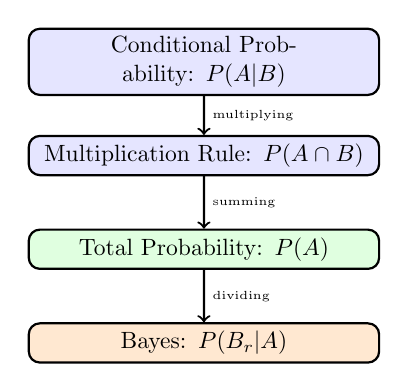
\begin{tikzpicture}[node distance=1.4cm, auto, thick, scale=0.85, transform shape]
                \node (P1) [draw, rounded corners, fill=blue!10, text width=5cm, align=center]
                {Conditional Probability: \(P(A|B)\)};
                \node (P2) [draw, rounded corners, fill=blue!10, below of=P1, text width=5cm, align=center]
                {Multiplication Rule: \(P(A\cap B)\)};
                \node (P3) [draw, rounded corners, fill=green!12, below of=P2, text width=5cm, align=center]
                {Total Probability: \(P(A)\)};
                \node (P4) [draw, rounded corners, fill=orange!18, below of=P3, text width=5cm, align=center]
                {Bayes: \(P(B_r|A)\)};

                \draw[->] (P1) -- (P2) node[midway,right,font=\tiny] {multiplying};
                \draw[->] (P2) -- (P3) node[midway,right,font=\tiny] {summing};
                \draw[->] (P3) -- (P4) node[midway,right,font=\tiny] {dividing};
            \end{tikzpicture}
            \end{center}
        \end{column}
        \begin{column}{0.48\textwidth}
            \small
            \textbf{Meaning of arrows + place of independence:}
            \begin{enumerate}
                \item From conditional probability, we find intersection by \textbf{multiplying}.
                \item If there is \textbf{independence}, step 1 simplifies: \(P(A\cap B)=P(A)P(B)\).
                \item In \textbf{total independence}, multiplication rule required in all subsets for 3+ events.
                \item We obtain general $P(A)$ by \textbf{summing} intersections.
                \item We return from observation to source by \textbf{dividing} by $P(A)$ (Bayes).
            \end{enumerate}

            \vspace{0.3cm}
            \textit{Each step uses the result of the previous one.}
        \end{column}
    \end{columns}
\end{frame}

\begin{frame}{Which Method in Which Question?}
    \begin{block}{Quick decision list}
        \begin{enumerate}
            \item ``A and B together/sequential'' \(\Rightarrow\) Multiplication rule
            \item ``General probability of X'' and multiple scenarios \(\Rightarrow\) Total Probability
            \item ``X observed, what is source?'' \(\Rightarrow\) Bayes
            \item ``Independent?'' \(\Rightarrow\) Compare \(P(A\cap B)\) with \(P(A)P(B)\)
        \end{enumerate}
    \end{block}
\end{frame}

\begin{frame}[fragile]{Mini-Quiz: Identify the Method}
    \begin{itemize}[<+->]
        \item ``Probability of being both red and defective?'' \(\Rightarrow\) Intersection/Multiplication
        \item ``Combine defective probability from three lines?'' \(\Rightarrow\) Total Probability
        \item ``Product known to be defective came from which line?'' \(\Rightarrow\) Bayes
        \item ``Can two disjoint events be independent?'' \(\Rightarrow\) No, if probability is positive
    \end{itemize}
\end{frame}

\begin{frame}{Exit Ticket: Self Check at Home}
    \begin{block}{3 short questions}
        \begin{enumerate}
            \item Can you clearly show the partition selection in the question?
            \item Can you explain the difference between \(P(A|B)\) and \(P(B|A)\) with an example?
            \item Do you test if the result is reasonable in real life?
        \end{enumerate}
    \end{block}
\end{frame}

\section{References}
\begin{frame}[allowframebreaks]{References}
    \nocite{*}
    \printbibliography{}
\end{frame}

\appendix
\section{Appendix: AI Assistant}
\begin{frame}{Your AI Assistant: NotebookLM}
    \begin{columns}[T]
        \begin{column}{0.48\textwidth}
            \justifying{}
            \textbf{Interact with Course Materials!}
            
            All content of this course (presentations, papers, and notes) has been uploaded to Google's advanced AI assistant \textbf{NotebookLM}.
            
            \vspace{1em}
            \begin{itemize}
                \item \textbf{Instant Answers:} Ask what's on your mind.
                \item \textbf{Summaries:} Learn complex topics simply.
                \item \textbf{Audio Overview:} Listen to the lecture like a podcast.
            \end{itemize}
            
            \vspace{1.5em}
            \begin{center}
                {\setbeamercolor{button}{bg=red,fg=black}
                \href{https://notebooklm.google.com/notebook/2877371a-cb71-4895-90cc-3cb61434962b}{\beamerbutton{\rule[-4ex]{0pt}{11ex}\Large \textbf{Try It Now}}}}
            \end{center}
        \end{column}
        
        \begin{column}{0.48\textwidth}
            \centering
            \includegraphics[width=\textwidth, height=0.6\textheight, keepaspectratio]{figures/notebooklm.jpg}
        \end{column}
    \end{columns}
\end{frame}

\begin{frame}[plain,noframenumbering]
    \begin{tikzpicture}[remember picture,overlay]
        \node[anchor=center, at=(current page.center), inner sep=0pt] {
            \includegraphics[width=\paperwidth, height=\paperheight]{figures/combined_qrs.png}
        };
        \node[anchor=south, at=(current page.south), yshift=0.5cm, fill=white!95, rounded corners, inner sep=10pt, text width=0.95\paperwidth, align=center] {
            \Large \textbf{\textcolor{blue}{Follow Us!}} \\
            \vspace{0.3em}
            \small Join our community to reinforce topics with lecture replays (YouTube), join professional project networks (LinkedIn), and be instantly informed about campus announcements (Instagram).
        };
    \end{tikzpicture}
\end{frame}

\end{document}
